\chapter{A Multiagent System Approach to Grocery Shopping}
\label{ch2}

\section{Introduction}

Aided by information systems for analyzing customer buying data, supermarket chains continually alter the prices of items to maximize their profits. They do this by, in essence, experimenting on their customers. For example, the price of an item might be raised at one store until customers stop buying it. This maximum price is then used at all of the stores in the chain. The customers at the supermarkets, however, do not have any comparable information systems that might aid them in price comparisons and are often at the mercy of the stores. Most stores do not post their prices online, so that consumers have to visit each store to find the prices of groceries, which makes comparison shopping prohibitive.

Imagine an online system where customers could post the prices they paid for their groceries (this could be automated by querying the RFID tags of the items) and where a prospective shopper could enter a grocery list and obtain a pointer to the store with the lowest total price. This would enable comparison shopping for groceries and would render the customer-to-store interactions fairer. It would also encourage stores to offer their true prices to avoid driving away potential customers. However, the effort required from the consumers would be substantial. To make the effort reasonable and manageable, each customer could benefit from an agent that represented his/her interests and interacted with the agents of the other customers and, possibly, with store agents. We have shown this system in Figure \ref{ch2:fmodelgrocery}. In this system, agents representing humans in the left part of the figure upload product information to the central manager, which is represented by the black robot in the middle, and a database is used to store the information. To make it clear, the interaction between a customer who uses this system and his agent is drawn specifically on the right side of the figure, while the customer could be one of the humans who contribute the product information as shown in the left part of the figure. The customer asks his agent for suggestions, and his agent will query the database, get information from there and provide suggestions based on the information.   

\begin{figure}
\centering
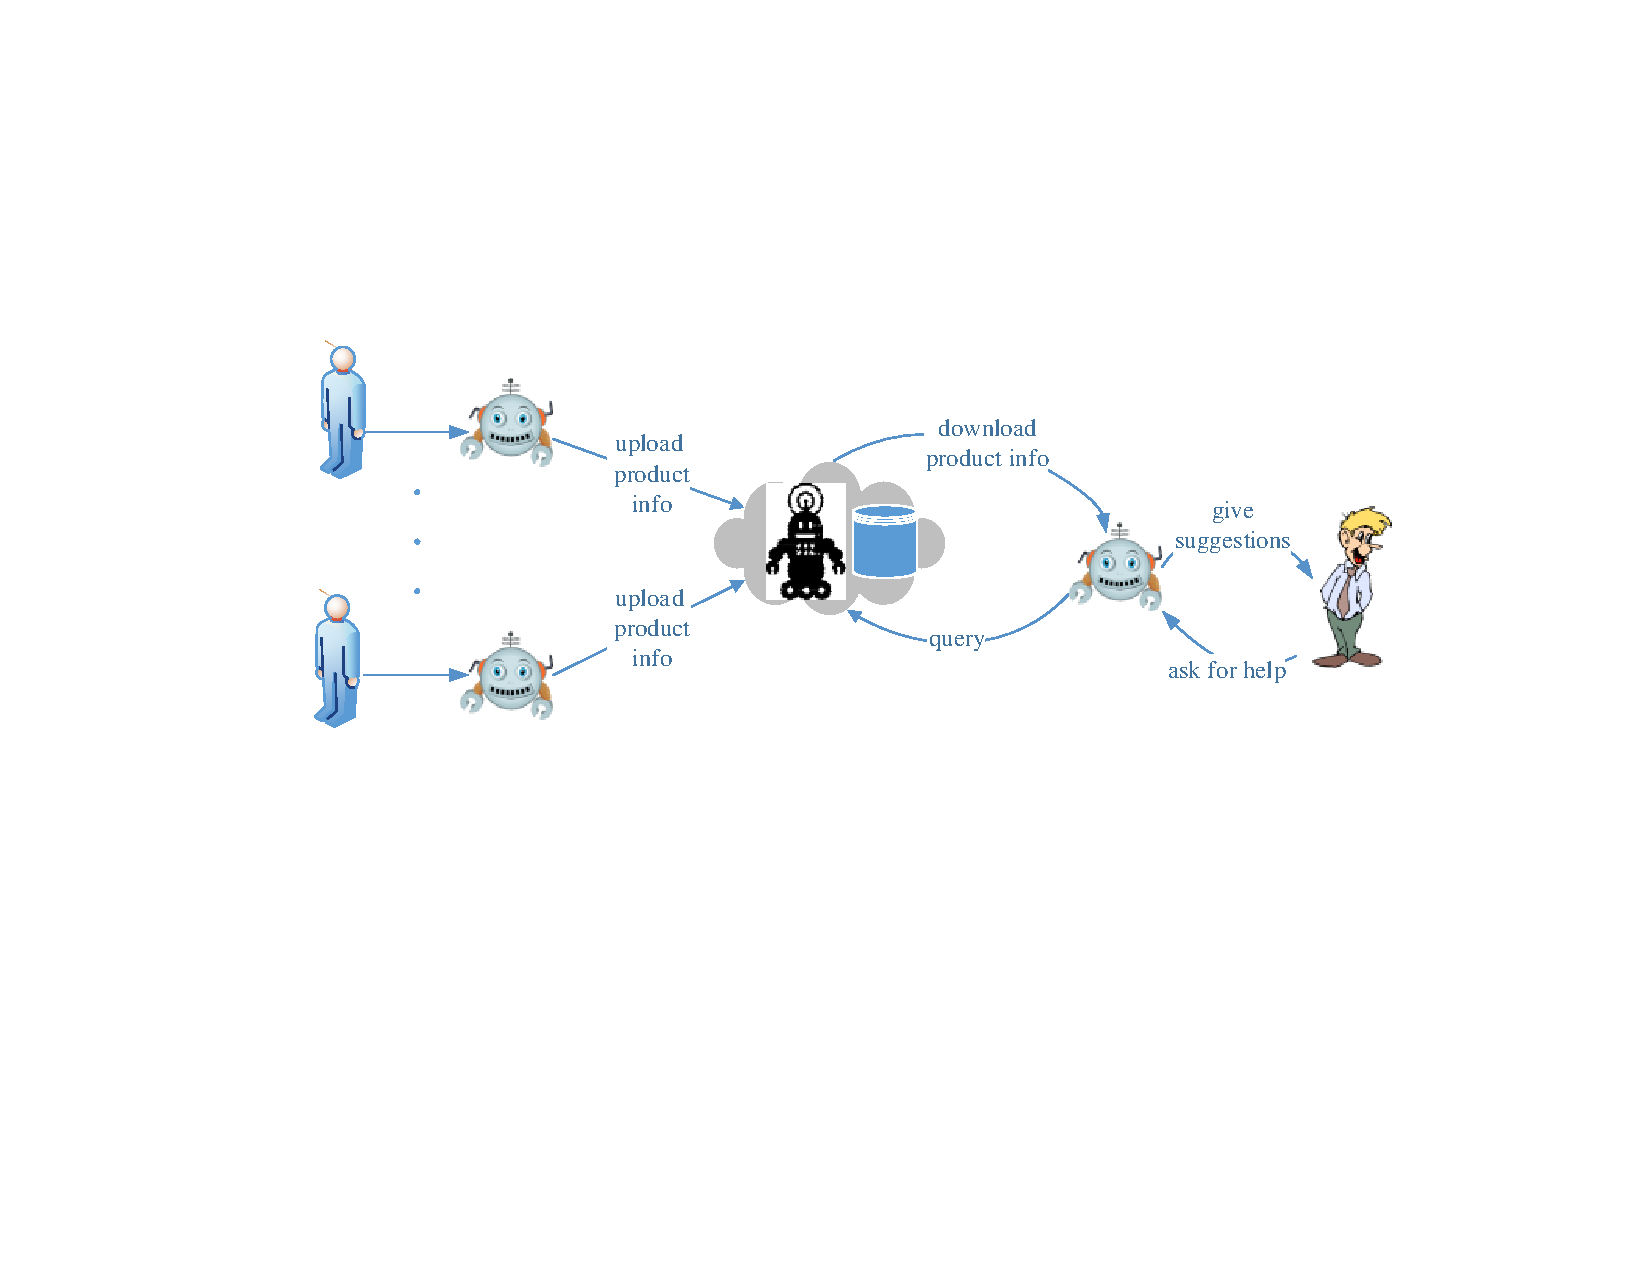
\includegraphics[scale=0.8]{chap2/chap2-model.pdf}
\caption{The model of the shopping system}
\label{ch2:fmodelgrocery}
\end{figure}

However, there is an expense in implementing and operating such a system. Moreover, its success is dependent on prices entered by other consumers, on the availability of goods, and on prices that stores might change to yield an advantage for them to the disadvantage of consumers. Hence, it is subject to errors and manipulation. To be feasible, the potential cost savings must substantially exceed the expense and effort of its implementation.

In this chapter, we investigate the efficacy of a consumer-oriented comparison-shopping system for groceries and the trade-offs in an implementation of it. Our approach is to use real data, normalize it according to typical consumer actions, and simulate a system of stores and consumers. We introduce both random and systematic (manipulation) errors into our simulation in order to evaluate its robustness.

Our assistant agent's objective is to assist a customer by all means, especially by providing a customer with the best combination of price and quality for a list of products available at different stores and making recommendations of store(s) optimal for shopping. The whole shopping procedure contains the following four steps, shown in Figure \ref{ch2:fgoal}. Note that the notation in this figure is from \cite{sterling2009}.
\begin{itemize}
\item[-]creating shopping list: a customer creates a shopping list based on his/her needs. He should specify items/products and the quantities of the items. 
\item[-]finding stores: find a series of available stores according to store hours, locations, the customer's preference and other possible factors.
\item[-]deciding stores: decide which store(s) to go to with the help of an assistance agent.
\item[-]transacting: drive to the store(s) and make transactions.
\end{itemize}

\begin{figure}
\centering
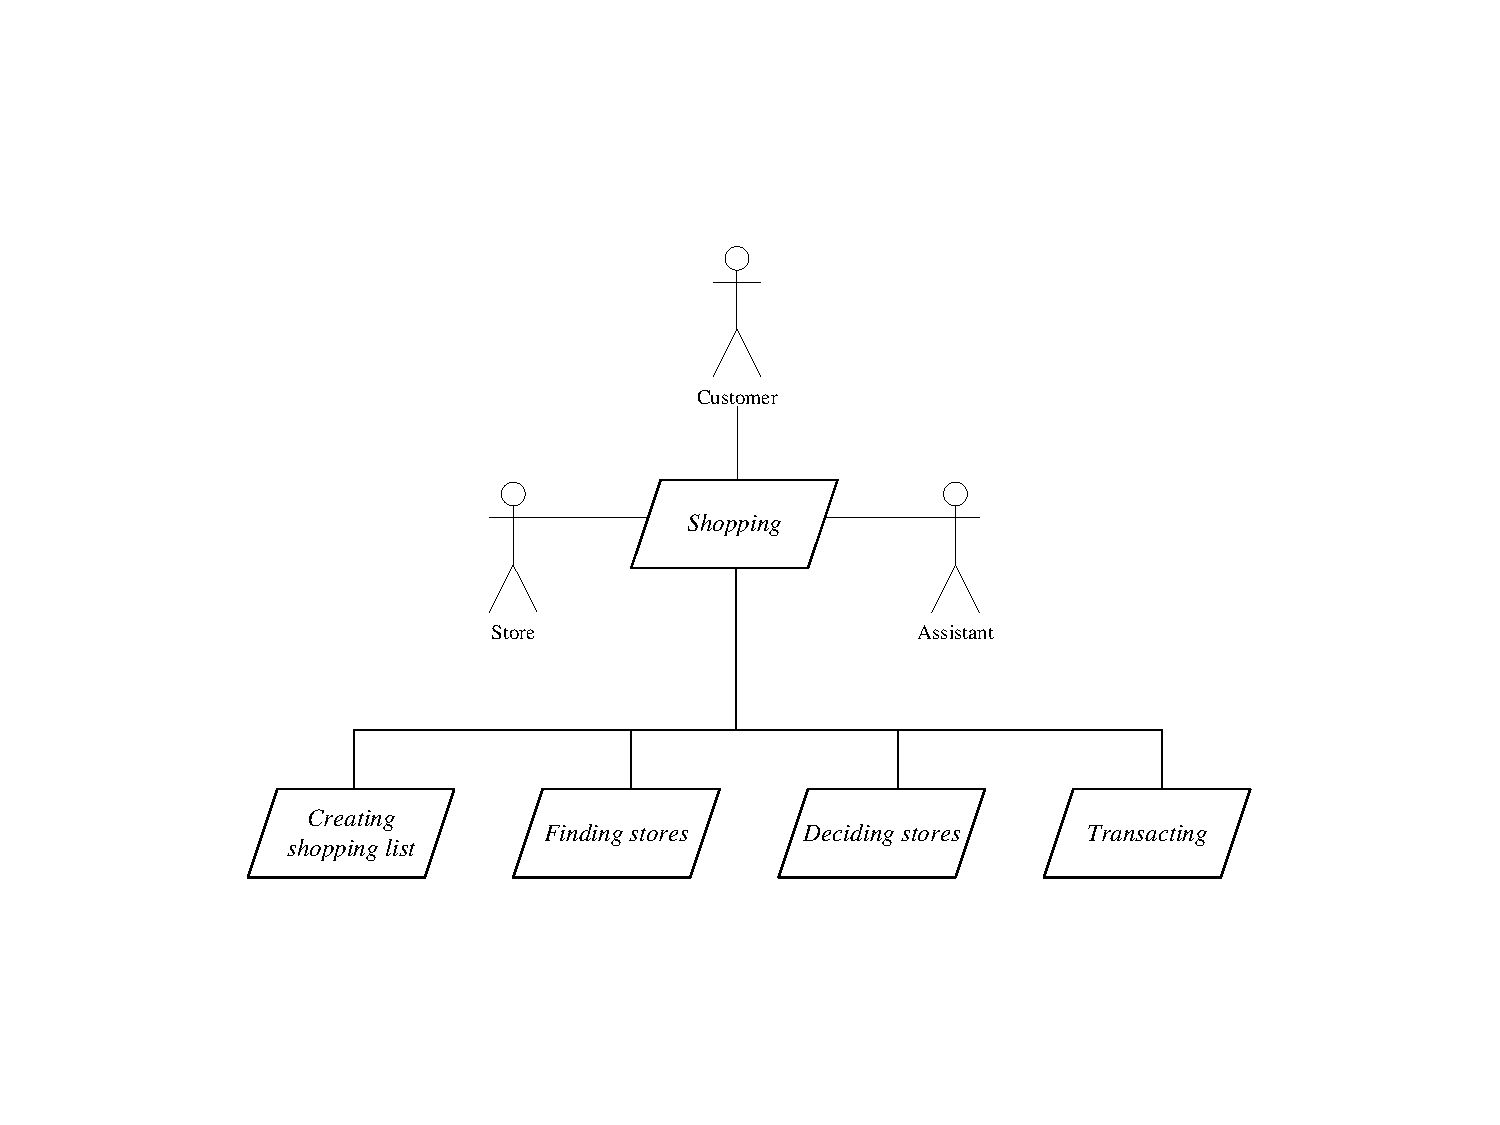
\includegraphics[scale=0.7]{chap2/chap2-goal.pdf}
\caption{Overall goal model}
\label{ch2:fgoal}
\end{figure}

\section{Background}

Price comparison services (also known as comparison shopping services) allow people to query a product's prices at online stores. The services list the product's prices in all of the stores and sort the prices to provide customers with support for their online shopping. An intelligent software agent to implement comparison shopping is called a shopbot \cite{clark2000}. 

In June 1995, the first well-known shopbot called BargainFinder \cite{bargainfinder} was released by a group of Andersen Consulting researchers as an intelligent software agent for comparison shopping. It was designed to find music CDs and had a rather simple interface. It allowed a user to enter the name of an artist and an album, searched eight online music stores, and displayed all CD prices on a web page. If the user clicked on the name of one of the stores, it would bring the user to the specific album on that store's website. Consumers gained obvious benefit from BargainFinder and it has been used widely. Nowadays, shopbots have greater functionality than before by including information about shipping expenses, taxes, vendors' rates, and product reviews. Some corporations even have their own shopbots, such as Google's Google Product Search and eBay's shopping.com. Recently there is also a mobile application for comparison shopping called RedLaser which can scan the barcode of a product by the phone's camera, search many online stores, and show their prices on the phone.

There are typically three steps for a shopbot to deal with data. First, it retrieves data from online stores or other shopbots, possibly by using an extraction method, such as \cite{yang2005}. Second, the data is processed according to a user's command. Last, the results are shown to the user on a webpage in a way that can be helpful to the user. One such system lets user re-rank the results locally \cite{buchholz2004}. Other researchers are developing better algorithms to improve the behavior of shopbots and making their performance more robust to changes in the stores' websites, such as by using Semantic Web concepts \cite{li2004}. Other related studies involve consumer search costs and benefits \cite{brynjolfsson2010} \cite{tang2010} and price-setting strategies \cite{greenwald2000}.

\section{Analysis and Simulation}

There are a number of variables in grocery shopping. Our simulation uses five parameters: customer input, customer location, store location, item price, and item quantity. Customer input is a customer shopping list that contains the items the customer wants to buy and the quantity of the items. Store location and customer location are used to calculate the fuel cost when driving to and from the stores. Item prices are those either reported by customers or by stores. We assume the quantity of a specific item in a store is either zero or infinity. All the prices are in US dollars. 

Our algorithm begins with the customer's shopping list of items and quantities. If the customer just goes to the stores with the lowest price for each item, the customer might need to go to many stores and spend more on fuel. So we search in all the stores and find the lowest price and the second lowest price of each item the customer wants to buy. The combinations of these two prices of the items may lead to the most economical way for shopping by reducing the fuel cost. We considered all the possibilities of combination of the two prices and calculate the total cost including grocery cost and the fuel cost. When calculating the fuel cost, we assume the customer goes to the nearest store he needs to go to where he has not already shopped until he gets all the items. For comparison, we also calculate the cost if the customer chooses to go to stores using three other strategies: (1) choose one store randomly and buy all the items at that store, (2) go to the nearest store, or (3) randomly go to one of the five nearest stores. Then we calculate the ratio of the grocery cost and the total cost of these three methods over that of our method to see the difference.

We next evaluate robustness. What if the stores claim their prices are lower than they actually charge if the stores themselves provide the prices? What if the customers make mistakes if they are responsible for reporting the prices to other customers? We also consider these two situations in our simulation.

%\begin{figure}
%\centering
%\includegraphics[scale=0.8]{chap2/chap2-.pdf}
%\caption{}
%\label{ch2:f}
%\end{figure} 
 
The NetLogo platform \cite{netlogo} has been proven to be a useful environment for agent-based simulations, such as supply chain simulation \cite{kawa2009}. We use it for our grocery shopping simulation. In our simulation, the number of stores and the number of items can be chosen by sliders in the Netlogo GUI, as shown in Figure \ref{ch2:fgui}. In reality, a customer will usually go to one of a few familiar supermarkets, which means we do not need to indicate very many stores. Our simulation has two phases.

\begin{figure}
\centering
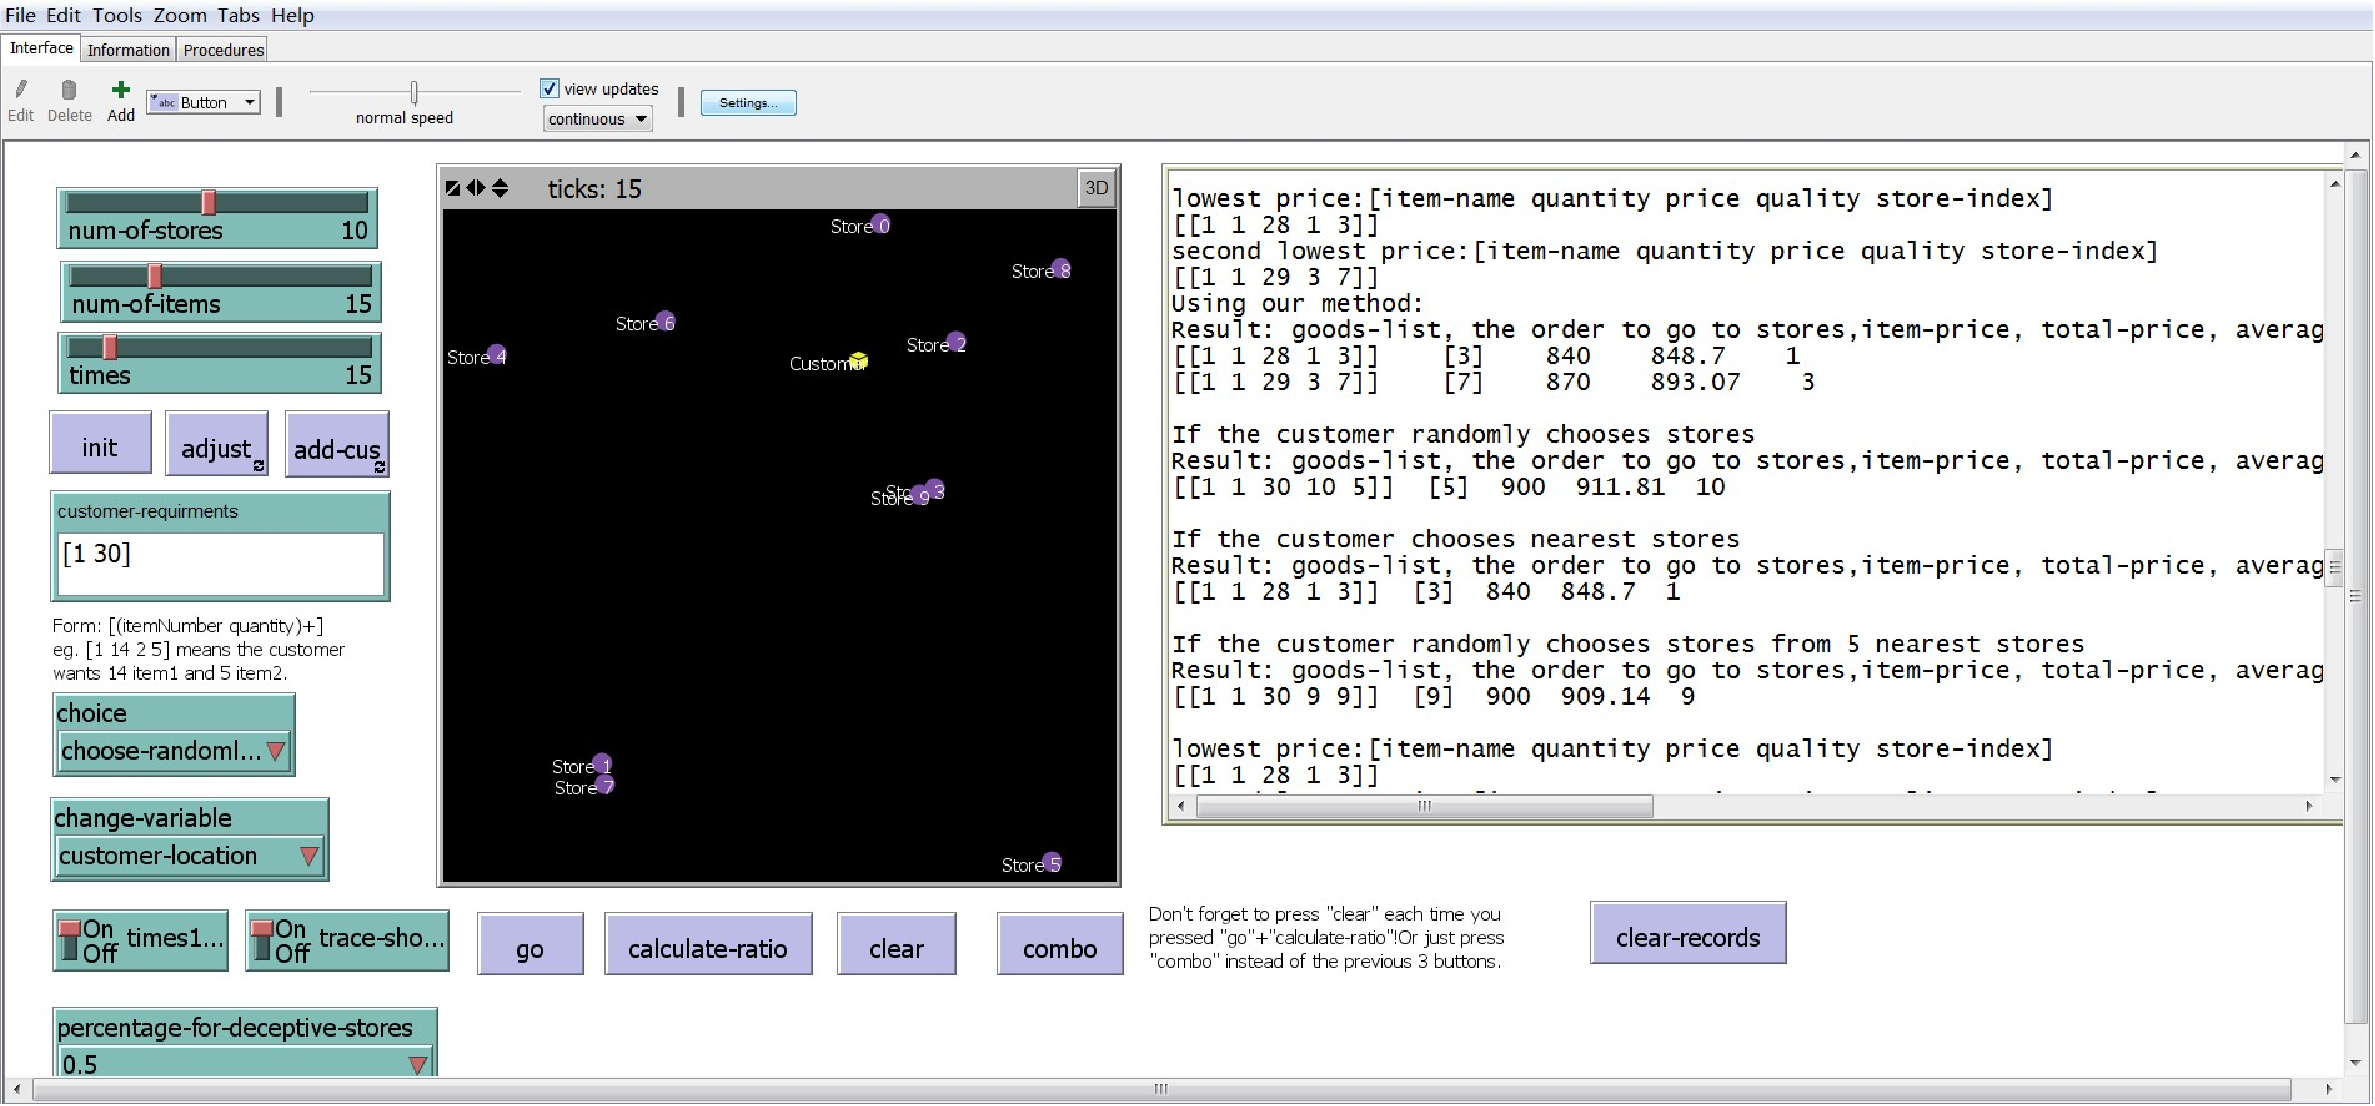
\includegraphics[scale=0.35]{chap2/chap2-fig2.pdf}
\caption{NetLogo GUI}
\label{ch2:fgui}
\end{figure} 

In the first phase, we simulate shopping according to fictitious prices generated randomly and examine the ratio of the cost of other methods over that of our method and evaluate the influence of different values for the parameters. For each combination of parameter values, we ran the simulation 100 times and used the mean of the 100 results. For deception, we assume that the deceptive stores say their prices are 10\% lower than the real prices and the percentage of deceptive stores are 25\%, 50\% and 75\% separately to see how it will affect the results.

In the second phase, we use realistic prices of items collected manually in the simulation and see whether there is a big difference between the results of simulation using fictitious prices and that of using realistic prices. With realistic prices, store location, item price, and item number are fixed. We did not consider the fuel cost in this part of the simulation, since its effect would be minor compared to the money spent on the items. As for the customer input, we constructed a shopping list according to the U.S. Consumer Price Index (CPI). CPI, which is published by the U.S. Bureau of Labor Statistics, measures a price change for a constant market basket of goods and services from one period to the next within the same area (city, region, or nation) \cite{blsglossary}. Along with CPI, the relative importance of components, which measures the importance of the items in the market basket by decimal numbers less than 1, is published. We created a realistic shopping list by selecting an item from each category according to its relative importance \cite{relativeimportance}. Since there are many categories, we did not include all of them in our shopping list, so the result was a list of 33 items. For these, we collected item price data from 5 different stores, as shown in Appendix \ref{app-table1}. We compared the saving of a customer going to two stores and that of just going to one store. To measure robustness, we checked the results if there was a 10\% possibility that the customers reported each digit of the prices wrong.

\section{Results and Discussion}

In our NetLogo Simulation, we assume there are 12 stores and 30 kinds of items in the stores. Given 10 items a customer wants to buy, we ran the simulation 100 times for a random change in a given parameter and calculated the mean, as shown in Tables \ref{ch2:t2} - \ref{ch2:t6}. In the tables, we represent the strategy of randomly going to one of the five nearest stores as "Choose randomly from 5". The ratios in the table are the ratio of the grocery cost or total cost of a certain method over that of our method. We also showed what items in which store the customer should buy. When simulating customers changing the items on their shopping list, using 30 kinds of items increases the program running time remarkably. To make this more manageable, we limit the simulation to 10 stores and 15 kinds of items.

\begin{table}[!t]

\centering
\caption{Simulation results of changing customer location}
\begin{tabular}{|c|c|c|}
\hline
\textbf{Method} & \textbf{Ratio of grocery cost}& \textbf{Ratio of total cost}\\ \hline
Choose randomly & 1.24 & 1.23\\ \hline
Choose nearest & 1.24 & 1.24\\ \hline
Choose randomly from 5& 1.22 & 1.22\\ \hline
\end{tabular}
\label{ch2:t2}
\end{table}

\begin{table}[!t]
\caption{Simulation results of changing store location}

\centering
\begin{tabular}{|c|c|c|}
\hline
%\multirow{2}{*}{\textbf{Method}} & \textbf{Ratio of}& \textbf{Ratio of}\\ 
%& \textbf{grocery cost}&  \textbf{total cost}\\\hline
\textbf{Method} & \textbf{Ratio of grocery cost}& \textbf{Ratio of total cost}\\ \hline
 Choose randomly& 1.24& 1.24\\ \hline
 Choose nearest& 1.24& 1.23\\ \hline
 Choose randomly from 5& 1.23& 1.23\\ \hline
\end{tabular}
\label{ch2:t3}
\end{table}

\begin{table}[!t]
\caption{Simulation results of changing item price}

\centering
\begin{tabular}{|c|c|c|}
\hline
\textbf{Method} & \textbf{Ratio of grocery cost}& \textbf{Ratio of total cost}\\ \hline
 Choose randomly& 1.22& 1.22\\ \hline
 Choose nearest& 1.22& 1.22\\ \hline
 Choose randomly from 5& 1.23& 1.22 \\ \hline
\end{tabular}
\label{ch2:t4}
\end{table}

\begin{table}[!t]
\caption{Simulation results of changing item number}

\centering
\begin{tabular}{|c|c|c|}
\hline
\textbf{Method} & \textbf{Ratio of grocery cost}& \textbf{Ratio of total cost}\\ \hline
 Choose randomly& 1.27& 1.26\\ \hline
 Choose nearest& 1.34& 1.33\\ \hline
 Choose randomly from 5& 1.30& 1.29\\ \hline
\end{tabular}
\label{ch2:t5}
\end{table}

\begin{table}[!t]
\caption{Simulation results of changing customer input}

\centering
\begin{tabular}{|c|c|c|}
\hline
\textbf{Method} & \textbf{Ratio of grocery cost}& \textbf{Ratio of total cost}\\ \hline
 Choose randomly& 1.18& 1.17\\ \hline
 Choose nearest& 1.11& 1.11\\ \hline
 Choose randomly from 5& 1.16& 1.16\\ \hline
\end{tabular}
\label{ch2:t6}
\end{table}

As can be seen from the tables mentioned above, our approach to deciding which stores to shop at can save 22\% or more in costs, except when changing customer input. Since we considered all possibilities and ran the simulation many times, it is safe to say that our approach is better than the other methods. As for changing the customer input, the savings are lower, possibly because the program generated the customer input randomly and it may contain fewer items.

We also considered deceptive stores. What if 25\%, 50\%, 75\% stores are deceptive by claiming that their price is 10\% lower than the real price? We ran the simulation with deceptive stores chosen randomly. The ratio in Table \ref{ch2:t7} shows the ratio of grocery cost or total cost of our approach using deceptive information over using actual information.

\begin{table}[!t]
\caption{Simulation results of deceptive stores}

\centering
\begin{tabular}{|c|c|c|}
\hline
\textbf{Percentage of}  & \multirow {2}{*}{\textbf{Ratio of grocery cost}}& \multirow {2}{*}{\textbf{Ratio of total cost}}\\ 
\textbf{deceptive stores}& & \\ \hline
 25\%& 1.02& 1.02\\ \hline
 50\%& 1.02& 1.02\\ \hline
 75\%& 1.01& 1.01\\ \hline
\end{tabular}
\label{ch2:t7}
\end{table}

The difference between the cost with real price data and that of deceptive price data is 2\% when 25\% of the stores are deceptive. The difference is smaller if more stores are deceptive: 1\% with 75\% deceptive stores. So when stores are deceptive, the customer will save less than when stores are honest. However, our approach is still valuable, because even after losing 2\% due to deception, the customer will still save more than 20\%.

Using the real price data we collected, Figure \ref{ch2:fcost1store} shows the total cost of the goods on the shopping list if a customer goes to just one store. The lowest price is \$114.27 from store 0.

\begin{figure}
\centering
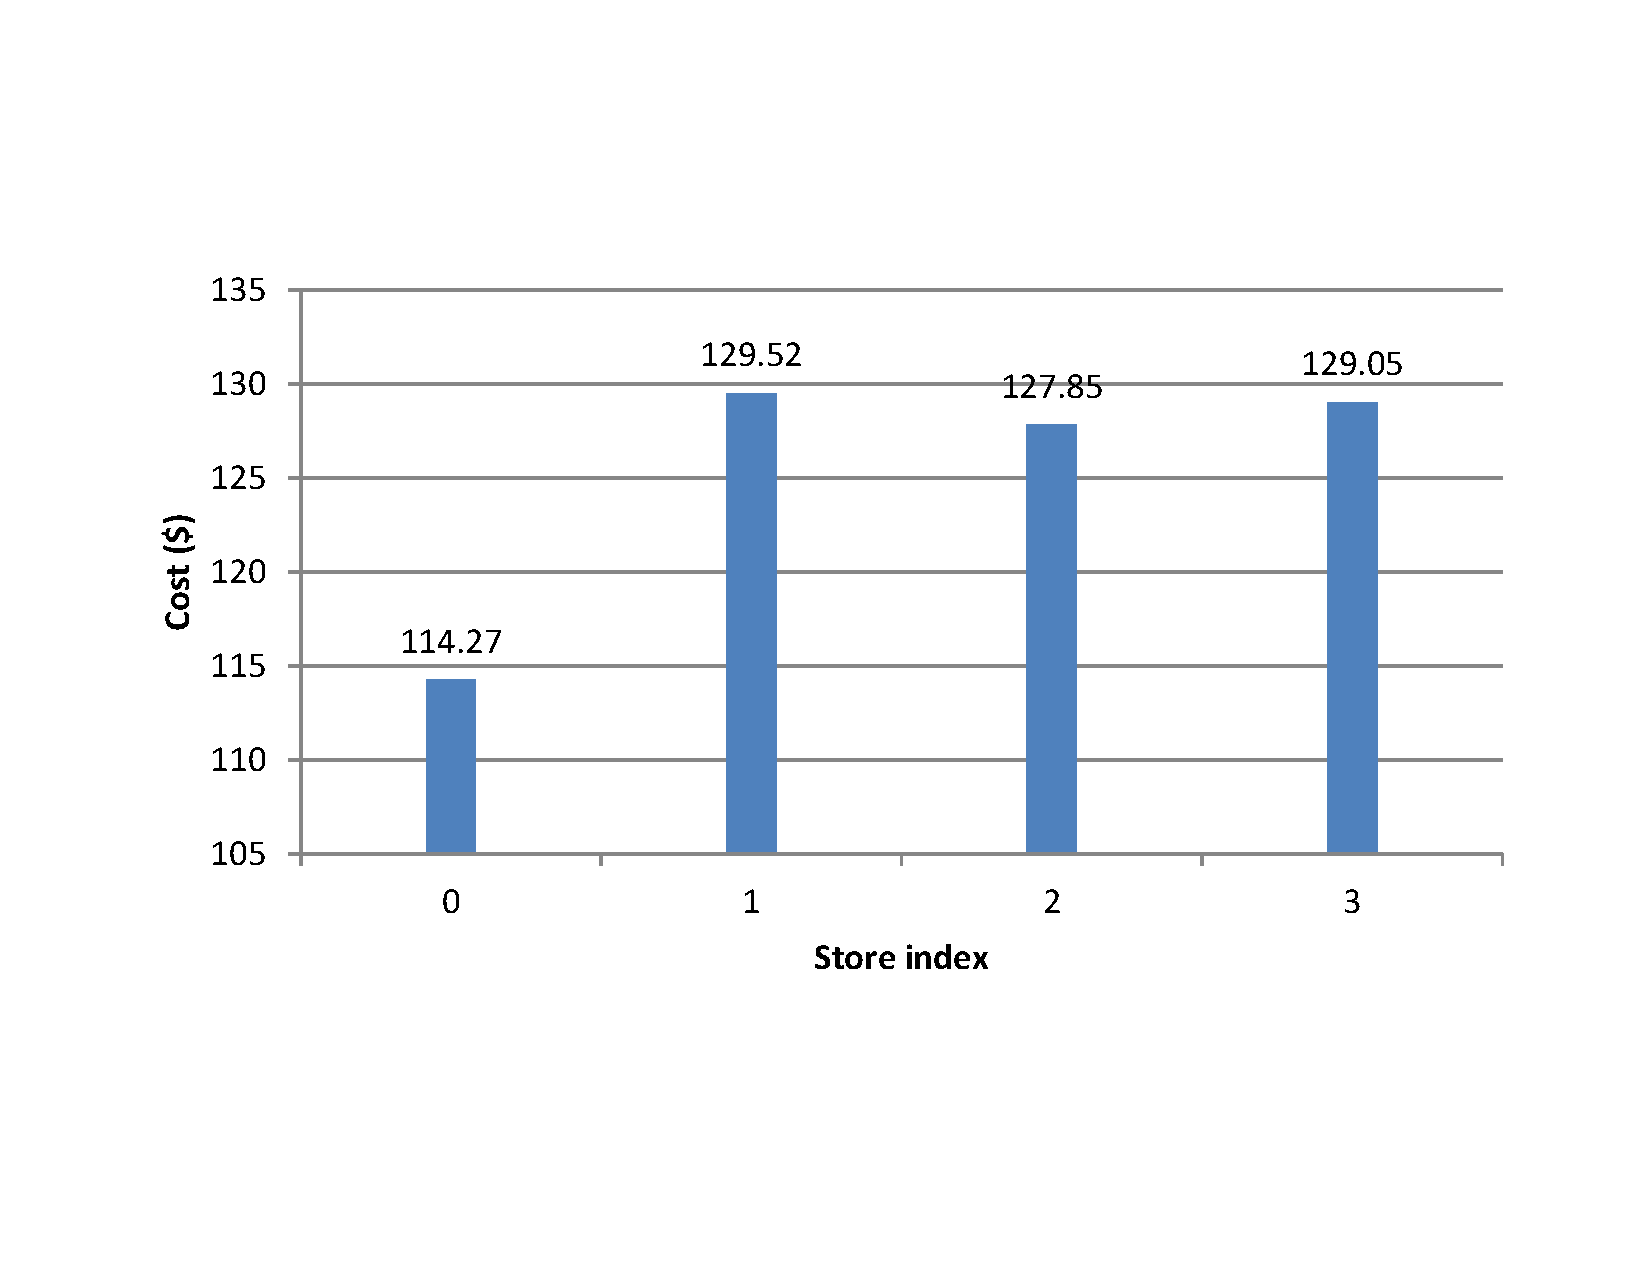
\includegraphics[scale=0.5]{chap2/chap2-cost1store.pdf}
\caption{Costs of shopping at one store}
\label{ch2:fcost1store}
\end{figure} 

The cost of buying each item at its lowest price is \$98.44, which is more than 13\% lower than going to one store, but a customer would have to go to four stores to get this lowest price. Because a customer might not want to go to more than two stores, we tried all combinations of two stores and calculated the cost. Figure \ref{ch2:fcost2store} shows that the lowest cost of \$106.58, which occurs when a customer shops at stores 0 and 4, is 6.7\% lower than going to just one store.

\begin{figure}
\centering
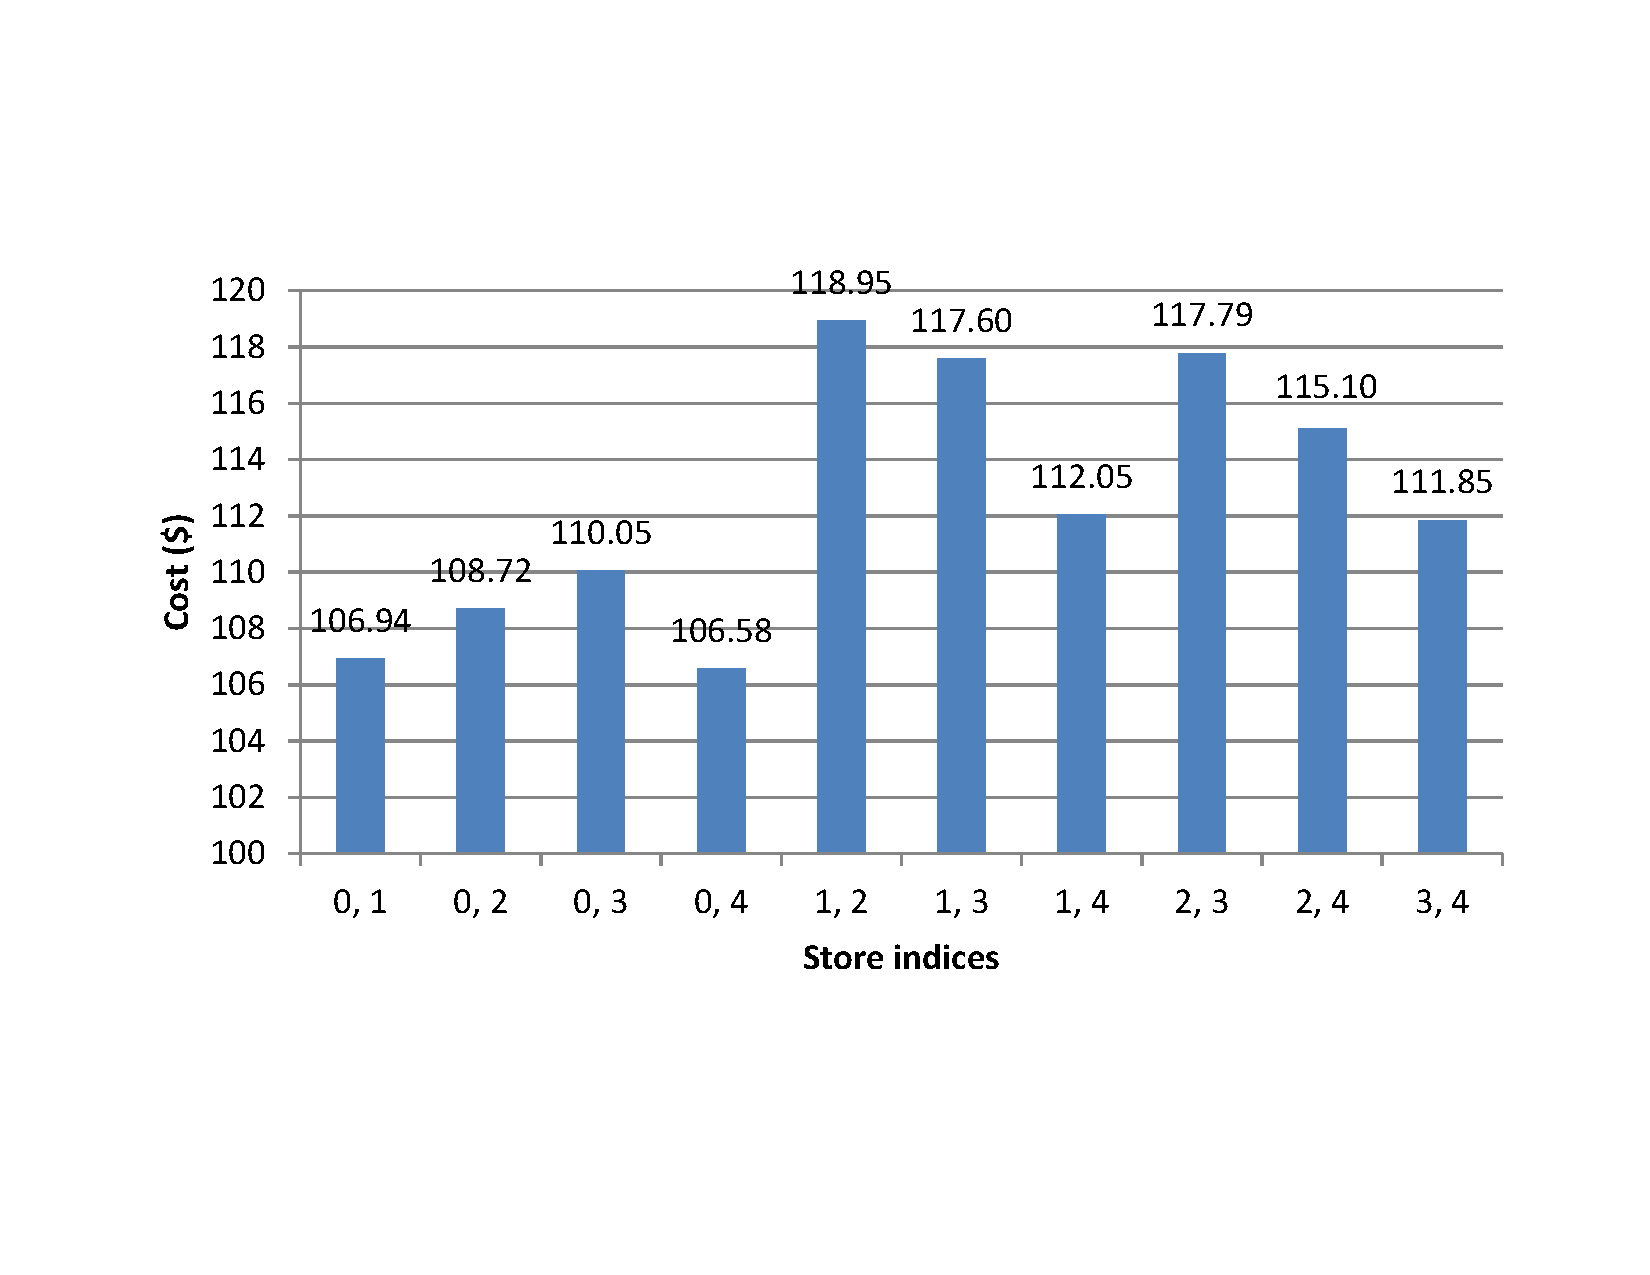
\includegraphics[scale=0.5]{chap2/chap2-cost2store.pdf}
\caption{Costs of shopping at two stores}
\label{ch2:fcost2store}
\end{figure} 

What if the customers reported the price data wrong? We simulated this situation by giving each digit of a price a 9\% possibility to change to other digits randomly, each with a 1\% possibility. When the price information is wrong, the only thing changed are the stores the customer would go to. When the customer arrives at the store, he will still pay the real price. We ran the simulation 500 times and the results are shown in Tables \ref{ch2:t10} and \ref{ch2:t11}, where "Frequency" means the number of simulations in which an agent recommends his principle to a certain store. Notice that some store or store combinations are never chosen in 500 simulations, because their overall costs are too high and thus can hardly be the lowest price, even with a 9\% possibility of incorrect price information. 

\begin{table}[!t]
\caption{Costs and frequencies of shopping at one store with reported price wrong}

\centering
\begin{tabular}{|c|c|c|}
\hline
\textbf{Store index} & \textbf{Cost (\$)}& \textbf{Frequency}\\ \hline
0& 114.27 & 489\\ \hline
2& 127.85 & 10\\ \hline
3& 129.05 & 1\\ \hline
\end{tabular}
\label{ch2:t10}
\end{table}

\begin{table}[!t]
\caption{Costs and frequencies of shopping at two stores with reported price wrong}

\centering
\begin{tabular}{|c|c|c|}
\hline
\textbf{Store indices} & \textbf{Cost (\$)}  &\textbf{Frequency}\\ \hline
 0, 4& 106.58& 315 \\ \hline
 0, 1& 106.94& 118\\ \hline
 0, 2& 108.72& 35\\ \hline
 0, 3& 110.05& 30\\ \hline
 3, 4& 111.85&2\\ \hline
\end{tabular}
\label{ch2:t11}
\end{table}

We can see from the tables that as for the results with one store, there is a 2\% possibility that the customer would go to another store due to the wrong price data, rather than going to the store with the lowest price. The average cost, after 500 simulation runs, is \$114.57, which is very close to \$114.27. For the results with two stores, there is a 37\% possibility that a customer would go to different stores other than the best combination of two stores. Though the possibility is significant, the average cost is \$107.04, which is very close to \$106.58, the lowest price possible for two stores. So on average, a customer can still save 6.3\% by going to two stores compared to going to just one store, even if the price data is incorrect.

\section{Conclusion}
A societal grocery shopping system as described in this chapter would be useful and practical, because it helps customers obtain a savings of 22\% or more according to our simulation. Even with deceptive pricing by stores or incorrect price data reported by other customers, it will still be helpful for obtaining some savings. During the simulation, we considered all the parameters that may vary in real shopping experiences: customer location, store location, item price, item number, and customer input. We varied the parameters to explore this five-dimensional space and produced results consisting of the average savings achieved by customers. To validate our results further, we also used real price data in a simplified version of our simulation containing fewer stores and shopping at just two of them. The results indicate an average savings of 6.7\% by choosing the best two stores. Even with incorrect price data, customers can still save 6.3\% on average. An implementation of our approach would require a social infrastructure where customers could report prices they discovered and find prices reported by others. Based on both simulated and real data, and the expected costs of such an infrastructure, our system would be useful and cost-effective in practice.